\documentclass[a4paper, 12pt]{article}
\usepackage{cmap}           % Пакет для поиска в полученной пдфке
\usepackage[utf8]{inputenc} % Ззамена кодировки файла на utf8
\usepackage[T2A]{fontenc}   % Подключение кодировки шрифтов
\usepackage[russian]{babel} % Использование русского языка 
\usepackage[left=2cm, right=2cm, top=1cm, bottom=2cm]{geometry} % Изменение размеров полей
\usepackage{indentfirst}    % Красная строка в начале текста
\usepackage{amsmath, amsfonts, amsthm, mathtools, amssymb, icomma, units, yfonts}
\usepackage{amsthm} % Пакет для нормального оформления теорем
\usepackage{algorithmicx, algorithm}
\usepackage{algpseudocode}
\usepackage{graphicx}
\usepackage{tikz}
\usepackage{esvect}
\usepackage{enumitem}
\usepackage{dcolumn}
\usetikzlibrary{calc,matrix}

%Теоремы
%11.01.2016
\newtheorem*{standartbase}{Теорема о стандартном базисе}
\newtheorem*{fulllemma}{Лемма}
\newtheorem*{sl1}{Следствие 1}
\newtheorem*{sl2}{Следствие 2}
\newtheorem*{monotonousbase}{Теорема о монотонном базисе}
\newtheorem*{scheme}{Утверждение 1}
\newtheorem*{n2}{Утверждение 2}
\newtheorem*{usp-rais}{Теорема Успенского-Райса}
\newtheorem*{rec}{Свойство рекурсии}
\newtheorem*{point}{Теорема о неподвижной точке}
\newtheorem*{zhegalkin}{Теорема Жегалкина}
\newtheorem*{poste}{Теорема Поста}
\newtheorem*{algo1}{Первое свойство алгоритмов}
\newtheorem*{vkliskl}{Формула включений и исключений}
\newtheorem*{baes}{Формула Байеса}
\newtheorem*{markov}{Неравенство Маркова}
\newtheorem*{existsFgthen2ndivn}{Теорема}
\newtheorem*{cantor}{Теорема Кантора}
\newtheorem*{cantorbern}{Теорема Кантора-Бернштейна}

%18.01.2016
\newtheorem*{theorem}{Теорема}

\renewcommand{\qedsymbol}{\textbf{Q.E.D.}}
\newcommand{\definition}{\underline{Определение:} }
\newcommand{\definitions}{\underline{Определения:} }
\newcommand{\definitionone}{\underline{Определение 1:} }
\newcommand{\definitiontwo}{\underline{Определение 2:} }
\newcommand{\statement}{\underline{Утверждение:} }
\newcommand{\note}{\underline{Замечание:} }
\newcommand{\sign}{\underline{Обозначения:} }
\newcommand{\statements}{\underline{Утверждения:} }

\newcommand{\Z}{\mathbb{Z}}
\newcommand{\N}{\mathbb{N}}
\newcommand{\Q}{\mathbb{Q}}
\newcommand{\R}{\mathbb{R}}



\begin{document}
\title{Дискретная математика.\\ Коллоквиум.}
\author{Лекторий ПМИ ФКН 2015-2016 \\ Доказательства 1 - 11, 19, 21, 35, 36, 40 -- Гринберг Вадим}
\date{16-21 марта 2016}

\maketitle

\part*{Доказательства}

\section*{1. Доказательство формулы включений и исключений.}

\begin{vkliskl}
Пусть у нас есть множества $A_1,\ A_2,\ \ldots,\ A_n$. Через
$S$ будем обозначать подмножество множества $\{1,\ \ldots,\ n\}$, каждое такое подмножество выделяет некоторое семейство подмножеств $\{A_i: i \in S\}$. Через $A_S$ обозначим
пересечение всех множеств, входящих в семейство $S$:

    \[
        A_S = \bigcap\limits_{i \in S}  A_i
    \]

Мощность множества, являющегося объединением этих множеств, находится по формуле:
    
    \[
        |A_1 \cup A_2 \cup \ldots \cup A_n| = \sum\limits_{S \neq \oslash} (-1)^{S + 1} |A_S|. 
    \]
    
\end{vkliskl}

\begin{proof}
Индукция по числу множеств. База индукции -- одно множество, формула очевидна: $|A| = (-1)^{1 + 1}|A|$.

Индуктивный переход использует формулу для количества элементов в объединении двух множеств:

\begin{multline*}
    |(A_1 \cup \ldots \cup A_{n - 1}) \cup A_n| = |A_1 \cup \ldots \cup A_{n - 1}| + |A_n| - |A_n \cap (A_1 \cup \ldots \cup A_n)| = \\ = |A_1 \cup \ldots \cup A_{n - 1}| + |A_n| - |(A_n \cap A_1) \cup \ldots \cup (A_n \cap A_{n - 1})|.
\end{multline*}

Для первого и третьего слагаемых по предположению индукции справедлива фор-
мула включений и исключений для $n - 1$ множества. Поэтому первое слагаемое дает вклад в сумму формулы для $n$ множеств вида

\[
    \sum_{\substack{S \neq \oslash \\ S \subseteq \{1,\ \ldots,\ n - 1\}}}(-1)^{|S| + 1}|A_S|
\]

Второе слагаемое -- это в точности $(-1)^{1 + 1}A_{\{n\}}$.

Рассмотрим теперь последнее слагаемое. По индуктивному предположению оно
равно

\[
    \sum_{\substack{S \neq \oslash \\ S \subseteq \{1,\ \ldots,\ n - 1\}}}(-1)^{|S| + 1}|B_S|
\]

где вместо множеств $A_i$ в формулу включений-исключений для $n - 1$ множества
подставлены множества $B_i = A_n \cap A_i$.

Для любого $S \subseteq \{1,\ \ldots,\ n - 1\}$ выполняется равенство

\[
    B_S = \bigcap\limits_{i \in S}(A_n \cap A_i) = A_n \cap A_S = A_{S\cup\{n\}}.
\]

Получается, что мощность объединения $|(A_1 \cup \ldots \cup A_{n - 1}) \cup A_n|$ представлена в виде суммы таких же слагаемых, что и в сумме формулы включений-исключений: первое слагаемое отвечает семействам, не содержащим $A_n$, второе и третье — семействам, содержащим $A_n$. Нужно ещё проверить, что эти слагаемые входят с правильными знаками. Для первых двух слагаемых это ясно из самих формул. Для третьего заметим, что мощность $S$ отличается от мощности $S \cup \{n\}$ на $1$, так как $S \subseteq \{1,\ \ldots,\ n - 1\}$. Это даёт лишний знак минус. Но в формулу для объединения двух множеств это слагаемое также входит со знаком минус. Поэтому окончательный знак будет правильным:

\[
    -(-1)^{|S|+1} = (-1)^{|S\cup\{i\}| + 1}.
\]

\end{proof}


\section*{2. Критерий существования функции, обратной к данной.}

\begin{theorem}
    Если для отображений $f : A \to B$ и $g : B \to A$ выполнены два равенства $g \circ f = id_A$ и $f \circ g = id_B$, то функция $f$ является биекцией и $g$ обратна к $f$.
\end{theorem}

\begin{proof}
    Пусть $f(x_1) = f(x_2)$. Тогда из первого условия на композиции
получаем:

\[
    x_1 = (g \circ f)(x_1) = g(f(x_1)) = g(f(x_2)) = (g \circ f)(x_2) = x_2.
\]

Значит, функция $f$ инъективна.

Для любого $y \in B$ из второго условия на композиции следует, что $y = f(g(y))$, то есть $y$ принадлежит множеству значений $f$. Значит, функция $f$ сюръективна.

Итак, $f$ биекция.

Если $y = f(x)$, то из первого условия на композиции получаем $g(y) = g(f(x)) = x$.

Значит, $g$ обратна к $f$.

\end{proof}

\section*{3. Количество функций из $n$-элементного множества в $k$-элементное.}

Положим $f : A \to B$, $|A| = n$, $|B| = k$. Для каждого элемента $x \in A$ есть $k + 1$ возможных значений для $f(x)$ (это значение может быть любым элементом множества $B$ или же не определено). Они выбираются независимо, так что всего есть $(k + 1)^n$ функций.

\section*{4. Количество всюду определенных функций из $n$-элементного множества в $k$-элементное.}

Положим $f : A \to B$, $|A| = n$, $|B| = k$. Для каждого элемента $x \in A$ есть $k$ возможных значений для $f(x)$ (это значение может быть любым элементом множества $B$). Они выбираются независимо, так что всего есть $k^n$ функций.

\section*{5. Количество инъективных отображений $n$-элементного множества в $k$-элементное.}

Положим $f : A \to B$, $|A| = n$, $|B| = k$. Если n > k, то их нет (большее множество не может быть инъективно отображено в меньшее).

Если $n \leq k$, то будем выбирать значения по очереди, расположив все $n$ элементов A в каком-то порядке. Для первого элемента допустимы все $k$ значений, для второго — все, кроме одного (уже использованного раньше), для третьего — $(k - 2)$ и так далее, всего получается $k(k - 1)(k - 2) \cdot \ldots \cdot (k - n + 1) = k!/(k - n)!$.

\section*{6. Количество сюръективных отображений $n$-элементного множества в $k$-элементное.}

\begin{theorem}

Положим $f : A \to B$, $|A| = n$, $|B| = k$. Количество сюръекций из $A$ в $B$ при $n \geq k$ равно

\[
    \sum\limits_{i = 0}^{k}(-1)^i {k \choose i} (k - i)^n
\]

и равно $0$ при $n < k$. Сюръекции должны быть определены на всех элементах.

\end{theorem}

\begin{proof}

Надо воспользоваться формулой включений и исключений. Пусть $B$ состоит из $k$ элементов $b_1,\ \ldots\ ,\ b_k$. Не-сюръекции $A \to B$ — это те функции, область значений которых не содержит одного из элементов $b_1,\ \ldots\ ,\ b_k$, то есть объединение множеств

\[
    A(b_1) \cup A(b_2) \cup \ldots \cup A(b_k),
\]

где через $A(b)$ обозначается множество тех функций, которые не принимают значения $b$. Легко понять, что все множества $A(b)$ имеют размер $(k - 1)^n$ (мы просто выбросили одно значение). Более того, столь же легко посчитать размер их пересечений: если $b \neq b'$, то $A(b) \cap A(b')$ — это функции, не принимающие значений $b$ и $b'$, их будет $(k - 2)^n$. Остаётся воспользоваться формулой включений и исключений: из всех функций ($k^n$) надо вычесть $n$ множеств вида $A(b_i)$, то есть $k(k - 1)^n$, затем вернуть обратно $k \choose 2$ их попарных пересечений, всего ${k \choose 2}(k - 2)^n$, затем снова вычесть тройные пересечения, которых ${k \choose 3}$ и каждое из которых имеет размер $(k - 3)^n$, и так далее.

\end{proof}


\section*{7. Формулировка и доказательство формулы включений и исключений для вероятностей.}

\begin{theorem}

Для всякой вероятностной модели и для произвольных множеств $A_1,\ \ldots\ ,\ A_n \subseteq U$ верно

\[
    Pr[A_1\cup A_2\cup \ldots \cup A_n] = \sum\limits_{i}Pr[A_i] - \sum\limits_{i < j}Pr[A_i \cap A_j] + \ \ldots \ = \sum\limits_{\oslash \neq I \subset \{1,\ 2,\ \ldots \ , \ n\}} (-1)^{|I| + 1} Pr \Biggl[\bigcap_{i \in I}A_i\Biggl]
\]

\end{theorem}

\begin{proof}

Индуктивное доказательство принципа включений
и исключений для множеств.

База для двух:

\begin{multline*}
    Pr[A_1 \cup A_2] = Pr [(A_1 \backslash A_2) \cup (A_1 \cap A_2) \cup (A_2 \backslash A_1)] = \\ = Pr[A_1 \backslash A_2] + Pr[A_1 \cap A_2] + Pr[A_2 \backslash A_1] = \\ = Pr[A_1 \backslash A_2] + 2 Pr[A_1 \cap A_2] + Pr[A_2 \backslash A_1] - Pr[A_1 \cap A_2] = \\ = Pr[A_1] + Pr[A_2] - Pr[A_1 \cap A_2],
\end{multline*}

Для доказательства шага индукции заметим, что

\begin{multline*}
    Pr [(A_1 \cup \ldots \cup A_{n - 1}) \cup A_n] = Pr [A_1 \cup \ldots \cup A_{n - 1}] + Pr[A_n] - Pr [A_n \cap (A_1 \cup \ldots \cup A_n)] = \\ = Pr [A_1 \cup \ldots \cup A_{n - 1}] + Pr[A_n] - Pr [(A_n \cap A_1) \cup \ldots \cup (A_n \cap A_{n - 1})].
\end{multline*}

Здесь мы воспользовались принципом включений и исключений для двух множеств. Осталось для каждого из объединений $A_1 \cup \ldots \cup A_{n - 1},\ (A_n \cap A_1) \cup \ldots \cup (A_n \cap A_{n - 1})$ воспользоваться предположением индукции.

\end{proof}

\section*{8. Формула Байеса.}

\begin{baes}
    Если вероятность событий $A$ и $B$ положительна, то
    
    \[
        Pr[A|B] = Pr[A] \cdot \frac{Pr[B|A]}{Pr[B]}
    \]

\end{baes}

\begin{proof}
    Запишем вероятность события $A \cap B$ через условные вероятности
двумя способами:

\[
    Pr[A \cap B] = Pr[B] \cdot Pr[A|B] = Pr[A] \cdot Pr[B|A].
\]

Теперь второе равенство даёт формулу Байеса.

\end{proof}

\section*{9. Формула полной вероятности.}

Пусть $B_1,\ \ldots\ ,\ B_n$ — разбиение вероятностного пространства $U$, то есть $U = B_1 \cup \ldots \cup B_n$, где $B_i \cap B_j = \oslash$ при $i \neq j$. Пусть также $Pr[B_i] > 0$ для всякого $i$. Тогда для всякого события $A$ из вероятностного пространства $U$

\[
    Pr[A] = \sum\limits_{i = 1}^n Pr[A|B_i] \cdot Pr[B_i].
\]

\begin{proof}
    
    \[
        Pr[A] = \sum\limits_{i = 1}^n Pr[A \cap B_i] = \sum\limits_{i = 1}^n Pr[A|B_i] \cdot Pr[B_i].
    \]
    
    Первое равенство получается по формуле сложения вероятностей непересекающихся событий (вероятность объединения независимых событий равна сумме вероятностей), а второе равенство – по определению условной вероятности.
    
\end{proof}

\section*{10. Линейность математического ожидания случайных величин.}

Пусть $f : U \to R$ и $g : U \to R$ – две случайные величины на одном и
том же вероятностном пространстве. Тогда

\[
    E[f + g] = E[f] + E[g].
\]

Другими словами, математическое ожидание линейно.

\begin{proof}
    Пусть вероятностное пространство $U$ состоит из исходов $u_1,\ \ldots\ ,\ u_k$ с вероятностями $p_1,\ \ldots\ ,\ p_k$ соответственно. Тогда по определению математического ожидания:
    
    \[
        E[f + g] = \sum\limits_{i = 1}^k (f(u_i) + g(u_i))p_i = \sum\limits_{i = 1}^k (f(u_i))p_i + \sum\limits_{i = 1}^k (g(u_i))p_i = E[f] + E[g].
    \]

\end{proof}

\section*{11. Формулировка и доказательство неравенства Маркова.}

\begin{markov}
    Пусть $f$ — случайная величина, принимающая только неотрицательные значения. Тогда для всякого $\alpha > 0$ верно
    
    \[
        Pr[f \geq \alpha] \leq \frac{E[f]}{\alpha}.
    \]

    То есть, вероятность того, что случайная величина $f$ сильно больше своего математического ожидания, не слишком велика.

\end{markov}

\begin{proof}
    По сути нужно доказать, что 
    
    \[
        E[f] \geq \alpha \cdot Pr[f \geq \alpha].
    \]
    
    Пусть случайная величина $f$ принимает значения $a_1,\ \ldots\ ,\ a_k$ с вероятностями \\ $p_1,\ \ldots\ ,\ p_k$. Запишем, чему равно её математическое ожидание по определению:
    
    \[
        E[f] = a_1p_1 + a_2p_2 + \ldots + a_kp_k.
    \]
    
    Посмотрим отдельно на те $a_i$, которые меньше $\alpha$, и отдельно на те $a_i$, которые не меньше $\alpha$. Если первые заменить на ноль, то сумма может только уменьшиться. Если вторые заменить на $\alpha$, то сумма также может только уменьшиться. После таких замен, у нас остаётся сумма нескольких слагаемых, каждое из которых есть $\alpha p_i$, где $p_i$ – вероятность некоторого значения случайной величины, не меньшего $\alpha$. Нетрудно видеть, что такая сумма как раз равна $\alpha \cdot Pr[f \geq \alpha]$, и теорема доказана.
    
\end{proof}

\section*{12. Полнота стандартного базиса.}

\begin{standartbase}

 Стандартный базис (базис, состоящий из операций отрицания, конъюнкции и дизъюнкции: $\{\neg, \vee, \wedge\}$) --- полный.
 
\end{standartbase}

\begin{proof}
Вспомним, что ДНФ - это дизъюнкция конъюнктов литералов. Построим схему ДНФ.

$x_1, \ldots ,x_n, \neg x_1, \ldots ,\neg x_n, c_1, \ldots ,c_n, D$, где $c_j$ --- конъюнкция литералов, $D$ --- дизъюнкция. Данный порядок действий соответствует определению ДНФ, следовательно ДНФ представима в виде схемы и любая функция представима в виде ДНФ, что доказано ранее. (Note: $0 = x \wedge \neg x, 1 = x \vee \neg x$)
\end{proof}

\section*{13. Существование булевых функций от n переменных схемной сложности $\Omega(2n/n)$.}

\begin{existsFgthen2ndivn}
    Существует функция $f: \{0, 1\}^n \rightarrow \{0, 1\}$
    такая, что $C(f) \geqslant \frac{2^n}{10n}$ 
    (в точности то же самое, что $C(f) = \Omega(\frac{2^n}{n})$).
\end{existsFgthen2ndivn}

\begin{proof}
    Воспоьзуемся мощностным методом. Всего булевых функций от $n$ аргументов $2^{2^n}$.

    Теперь узнаем, сколько булевых схем размера меньше либо равных некоторого фиксированного
    числа $L$. Для этого будем кодировать схемы двоичными словами. Посмотрим на 
    какое-то присваивание в схеме $S$: $g_k = g(g_i, g_j)$. Для кодирования
    самой функции $g$ нужно 2 бита (так как в стандартном базисе всего три функции).
    Для кодирования номеров аргументов $i$ и $j$ нужно битов не более, чем $log_2L$.
    А значит для всего присваивания $g_k$ нужно не более $2 \cdot (1 + log_2L)$ бит.

    Итого размер одной схемы в битах: $L \cdot 2 \cdot (1 + log_2L)$. Каждая схема
    кодирует ровно одну функцию. А значит каждое двоичное слово кодирует не более 
    одной функции (так как некоторые двоичные слова ни одну схему не задают).

    Получается и схем размера $L$ не более, чем двоичных слов для схем такой длины,
    то есть: $2^{2L(1 + log_2L)}$.

    Пусть $L = \frac{2^n}{10n}$. Размер схемы в битах тогда будет равен: 
    \[
    L_2 = \frac{2^n}{10n} \cdot 2 \cdot \left(1 + log_2\left( \frac{2^n}{10n} \right)\right) = 
    \frac{2^n}{5n} \left( 1 + n - log_2(10n) \right), 1 - log(10n) \leqslant 0 \implies
    L_2 \leqslant \frac{2^n}{5n}\cdot n = \frac{2^n}{5}
    \]
    А значит функций, задающейся схемой такой длины не более чем $2^{\frac{2^n}{5}}$.
    Нетрудно заметить, что это число значительно меньше числа функций от $n$ аргументов.
    
    \[
        2^{\frac{2^n}{5}} < 2^{2^n}
    \]

    А значит существует функция, задающаяся схемой длины больше, чем $L$.
    
\end{proof}

\section*{14. Верхняя оценка $O(n2^n)$ схемной сложности булевой функции от $n$ переменных.}

\begin{theorem}
    $C(f) = O(n \cdot 2^n)$
\end{theorem}

\begin{proof}
    Повторим предыдущие рассуждения при доказательстве того, что в стандартном
    базисе любая функция вычислима. Для этого вспомним сокращенную ДНФ:
    \[
    f(x) = \bigvee\limits_{\substack{a: f(a) = 1 \\ a \in \{0, 1\}^n}} x^a, \ 
    x^a = \bigwedge\limits_{i = 1}^{n} x_i^{a_i}
    \]
    Нетрудно посчитать, что схема для вычисления $x^a$ имеет размер $L_a = O(n)$.
    Тогда итоговый размер схемы $L \leqslant 2^n \cdot O(n) \iff L = O(n \cdot 2^n)$.
\end{proof}


\section*{15. Cхема сложения $n$-битовых чисел сложности $O(n)$.}

Вспомним схему для сложения по модулю (2 из определений). На каждом шаге добавлялось 5 присваиваний, значит, справедливо рекуррентное соотношение для количества операций $S_n = S_{n-1} + 5$. Из такого соотношения нетрудно сделать два вывода:
\begin{itemize}
    \item $S_n$ вычисляется за O(n).
    \item Из того, что $S_1$ --- константа, следует, что $S_n$ --- также константа.
\end{itemize}

Пусть у нас есть 2 двоичных числа $x : \{x_0, x_1, \ldots, x_{n-1}\}, y : \{y_0, y_1, \ldots, y_{n-1}\}$, где $x_0, x_1, \ldots, x_{n-1}, y_0, y_1, \ldots, y_{n-1}$ --- двоичные разряды. Нужно выполнить схему $f: \{0,1\}^{2n} \rightarrow \{0,1\}^{n+1}$, результатом которой является $z : {z_0, z_1, \ldots, z_n-1}$.

Вспомним привычный нам алгоритм сложения двоичных чисел поразрядно в столбик.

$\begin{array}{l c c r}
 C_n & C_{n-1} & \ldots & C_0 \\
 \hline 0 & x_{n-1} & \ldots & x_0 \\
        0 & y_{n-1} & \ldots & y_0 \\
 \hline z_n & z_{n-1} & \ldots & z_0 \\
\end{array}$

Обратим внимание на присутствие $C_0, \ldots, C_n$. Они являются тем числами (0 или 1) которые мы "запоминаем" при сложении и переносим на следующий разряд. Теперь рассмотрим отдельно некоторый $i$-й разряд сложения.

$\begin{array}{l}
 C_i \\
 \hline x_i \\
        y_i \\
 \hline z_i = x_i \oplus y_i \oplus c_i \\
\end{array}$

Нетрудно догадаться, что $z_i$ является суммой по модулю 2 $i$-х разрядов 2 слагаемых и "запомненного" числа от предыдущих разрядов. Возникает вопрос, как схемно выразить $c_{i+1}$ через предыдущие разряды? Оказывается, это также нетрудно сделать, воспользовавшись функцией MAJ: $c_{i+1} = MAJ(x_i, y_i, c_i)$.

Теперь поговорим о размере такой схемы. Как мы знаем из предыдущей лекции, сложение по модулю 2 и функцию большинства можно выполнить за константное число присваиваний. Получается, для операций $S_n, S_{n-1}$ справедливо рекуррентное соотношение $S_n = S_{n-1} + C$, где $C$ --- некая константа. Из этого можно сделать вывод, что $S_n$ вычисляется за $O(n)$.

\section*{16. Cхема умножения $n$-битовых чисел сложности $O(n^2)$.}

Вспомним "школьную" схему умножения столбик. Как мы помним, нужно сначала посчитать результаты поочередного умножения разрядов $y$ на все разряды $x$: 

\[u_i = y_i(x_0, x_1, \ldots, x_n)\]

Операция выполняется за $n \cdot O(n) = O(n^2)$.

Далее мы складываем получившиеся произведения $u_0 + u_1 + \ldots + u_n$. Операция выполнится за $O(n) \cdot O(2n) = O(n^2)$. Итого получаем выполнимость операции за $O(n^2)$.

\section*{17. Схема проверки связности графа на $n$ вершинах полиномиального размера.}

\textit{Проверка неориентированного графа на связность}: $Conn: \{0,1\}^{n \choose 2} \rightarrow \{0,1\}$.

Пусть булева переменная $x_{ij}, \{i,j\} \in F(G)$ принимает заначение 1 в том случае, если между вершинами $i$ и $j$ есть ребро. Рассмотрим функцию от таких булевых переменных.

Зададим \textit{матрицу смежности} графа. Это матрица $A \in {0, 1}^{n \times n}$, в которой на пересечении строки $i$ со столбцом $j$ стоит 1 тогда и только тогда, когда данные вершины связаны ребром. Такую матрицу и подадим на вход функции $Conn$. Заметим, что матрица смежности симметрична и на диагонали у нее обязательно стоят нули (мы запрещали петли --- ребра, ведущие из вершины в нее же саму).

\[A = \begin{pmatrix} 0 & \ldots & x_{1n} \\ x_{21} & \ldots & x_{2n} \\ \vdots & \ddots & \vdots \\ x_{n1} & \ldots & 0 \end{pmatrix}\]  

Рассмотрим матрицу $A'$, которая отличается от матрицы $A$ тем, что у нее на главной диагонали стоят единицы, а не нули (в остальном
матрицы совпадают).В терминах графов это означает, что к каждой вершине мы добавляем петлю. В модели простых неориентированных графов мы этого не допускали, но ничего не мешает нам рассмотреть графы с петлями. Идея состоит в том, что теперь, если между двумя вершинами есть путь длины меньше $n - 1$, то есть и путь длины ровно $n - 1$ (достаточно добавить к пути нужное количество петель). Нам достаточно взглянуть на $(A')^{n - 1}$. Если в ячейках этой матрицы нет нулей, то граф связен, иначе не связен. 

\[A' = \begin{pmatrix} 1 & \ldots & x_{1n} \\ x_{21} & \ldots & x_{2n} \\ \vdots & \ddots & \vdots \\ x_{n1} & \ldots & 1 \end{pmatrix}\]

Также упрощение можно провести со способом возведения матрицы в степень. В данный момент мы это делаем над действительными числами, что заставляет нас складывать и умножать целые числа. Чтобы делать это с помощью схем, нам придется использовать описанные выше схемы для сложения и умножения, а чтобы оценить размер получившейся схемы придется оценивать величину возникающих в процессе
вычислений целых чисел. Все это не очень хочется делать. Решение состоит в том, чтобы вместо умножения матриц над целыми числами воспользоваться так называемым \textit{булевым умножением матриц}. В нем формулы для умножения матриц такие же, как и в обычном умножении, только вместо операции умножения используется конъюнкция, а вместо сложения --- дизъюнкция. Тогда можно по индукции доказать, что в (булевой) матрице $A'^k$ на пересечении строки $i$ и столбца $j$ стоит 1 тогда и только тогда, когда в графе есть путь из вершины $i$ в вершину $j$ длины не больше $k$. Теперь мы готовы описать схему для проверки графа на связность. На вход схема
(по существу) получает матрицу смежности $A'$. Схема последовательно вычисляет булевы степени этой матрицы $A'^2, \ldots A'^{n - 1}$. Затем схема вычисляет конъюнкцию всех ячеек матрицы $A'^{n - 1}$ и подает ее на выход. 

Оценим размер получившийся схемы. Для булева умножения двух булевых матриц размер $n \times n$ достаточно $n^2 \cdots O(n) = O(n^3)$ операций (каждая ячейка произведения матриц вычисляется за линейное число операций, всего ячеек $n^2$). Всего нам нужно $(n - 1)$ умножение матриц, так что для вычисления матрицы $A'^{n - 1}$ достаточно $O(n^4)$ операций. На последний этап (конъюнкция ячеек $A'^{n - 1}$ нужно $O(n^2)$ операций, итого получается $O(n^4) + O(n^2) = O(n^4)$ операций.

\section*{18. Подмножество счетного множества конечно или счетно.}

\label{prop:AsubsetA}
            $A$ -- счётное множество. Тогда $A' \subseteq A$ счётно или конечно.
            \begin{proof}
                $A = \{a_0, a_1, \ldots, a_n, \ldots\}$. Вычеркнем все элементы, в $A'$
                не входящие. $A' = \{a_{j_0}, a_{j_1}, \ldots, a_{j_n}, \ldots\}$.

                Если последовательность $\{a_{j_n}\}$ конечна, то и $A'$ конечно.
                Если она бесконечна, то $A'$ очевидно счётно.
            \end{proof}

\section*{19. Любое бесонечное множество содержит счетное подмножество.}

\statement{Любое бесконечное множество содержит счетное подмножество.}

\begin{proof}
    Пусть $A$ -- бесконечное множество. Тогда $M \neq \oslash$. Выберем какой-нибудь из его элементов и обозначим его через $a_1$. Допустим в $A$ уже выбраны $n$ попарно различных элементов $a_1,\ a_2,\ \ldots\ ,\ a_n$. Так как $M$ бесконечно, то
    
    \[
        A \backslash \{a_1,\ a_2,\ \ldots\ ,\ a_n\} \neq \oslash
    \]
    
    и можно выбрать $a_{n + 1} \in A \backslash \{a_1,\ a_2,\ \ldots\ ,\ a_n\}$.
    
    Он отличен от всех ранее выбранных элементов. 
    
    Таким образом, по индукции доказывается, что для любого $n$ существует в $A$ подмножество $A_n = \{a_1,\ a_2,\ \ldots,\ a_n\}$ из $n$ элементов, причем множество $A_{n + 1}$ получается из $A_n$ присоединением одного нового элемента $a_{n + 1}$. Ясно, что объединение
    
    \[
        B = \bigcup\limits_{n = 1}^{\infty}A_n = \{a_1,\ a_2,\ \ldots\ ,\ a_n,\ \ldots \ \}
    \]
    
    является счетным подмножеством $A$.
    
\end{proof}

\section*{20. Счетное объединение конечных или счетных множеств конечно или счетно.}

        $\{A_0, A_1, \ldots, A_n, \ldots\} = \mathfrak{F} \sim \N$. $A_i$ -- множество.
        $\mathfrak{F}$ называется семейством множеств. 
        $A = \bigcup\limits_{i=0}^{\infty} A_i$.

        \statement $A$ -- счётно.
        \begin{proof}
        \begin{align*}
            A_0 &= (a_{00}, a_{01}, \ldots, a_{0n}, \ldots) \\
             A_1 &= (a_{10}, a_{11}, \ldots, a_{1n}, \ldots) \\
        \end{align*}
               Некоторые из множеств могут быть конечны. Дополним их до счётных
               пустым символом $\lambda \notin A$.

               Построим последовательность: $a_{00}, a_{01}, a_{10}, a_{02},
               a_{11}, a_{20}, \ldots$. (то есть проходим последовательно все значения
               сумм индексов от $0$ до $\infty$).

               Теперь исключим из последовательности повторения и символы $\lambda$.
               Получим требуемую последовательность $(a'_0, a'_1, \ldots, a'_n, \ldots)$.

               Теперь получим функцию $f: [n] \to A$ или $f: \N \to A$. $f$ -- биекция.
               В первом случае множество конечно, во втором счётно.

               Можно было бы и не вводить $\lambda$, а исключать эти элементы сразу,
               но так проще (нет никаких условий).
        \end{proof}


\section*{21. Счетность декартова произведения счетных множеств.}

\label{prop:CartProdAB}
          Декартово произведение счётных множеств счётно.
          Напомним, что \[A \times B = \left\{ (a; b)\ |\ a \in A, b \in B \right\}\]
          \begin{proof}
              По определению декартово произведение есть множество всех упорядоченных пар вида $\langle a,\ b\rangle$, в которых $a \in A$ и $b \in B$. Разделим пары на группы, объединив пары с одинаковой первой компонентой (каждая группа имеетвид $\{a\} \times B$ для какого-то $a \in A$). Тогда каждая группа счётна, поскольку находится во взаимно однозначном соответствии с $B$ (пара определяется своим вторым элементом), и групп столько же, сколько элементов в $A$, то есть счётное число.
          \end{proof}

\section*{22. Счетность множества слов в конечном или счетном непустом алфавите.}

Что такое слова длины $n$ в алфавите $A$?
Это в точности декартова степень $A^n$.

Каждая такая степень либо счётна (если $A$
счётно), либо конечна (если $A$ конечно).

Что такое тогда множество всех слов в алфавите?
Это в точности объединение всех слов длины $0, 1, 2, \ldots, n, \ldots$:
\[
    A^* = \bigcup\limits_{i \in \N}A^i
\]

Получили счётное объединение счётных или конечных множеств
(а оно счётно или конечно).
 
Доказательство этих фактов есть в свойствах счётных
множеств (документ с определениями). Странно? Ну ладно,
чёрт его знает как так получилось :).

\section*{23. Несчетность множества мощности континуум.}

Определим действительные числа следующим образом: сопоставим каждому $x \in \R$ двоичное число: $\pm \lefteqn{\underbrace{\phantom{10110 \dots 1011}}_{\text{целая часть}}}10110 \dots 1011 .\overbrace{110001 \dots 00110}^{\text{дробная часть}}$. Считаем известным, что ряд из каких-то степеней двоек сходится, причём запрещаем в числах данного вида "хвосты из единиц".

Множество имеет мощность континуум, если оно равномощно $\R$.

Множество счётно, если оно равномощно $\N$.
\\

\begin{cantor}
    $\N \nsim \R$
\end{cantor}

\begin{proof}

Воспользуемся тем, что $\R \sim 2^{\N}$, и докажем $\N \nsim 2^{\N}$ для получения требуемого.
    
    Диагональное рассудение:
    
    Пусть $F = \{f_0, f_1, \ldots , f_n, \ldots \}$ -- множество последовательностей $f \in 2^{\N}$. Покажем, что $\exists x \in 2^{\N} : x \notin F$, тем самым доказав, что отображение $\N \to 2^{\N}$ не сюръективно.
    
    Запишем элементы $F$ в квадратную таблицу по правилу $f_i = \{f_{i0} \ f_{i1} \ldots f_{in}\}$:
    
    $\begin{array}{lcccr}
        f_0 = & f_{00} & f_{01} & \ldots & f_{0n}\\
        f_1 = & f_{10} & f_{11} & \ldots & f_{1n}\\
        \vdots & \vdots & \vdots & \ddots & \vdots \\
        f_n = & f_{n0} & f_{n1} & \ldots & f_{nn}\\
    \end{array}$
    
    Выпишем последовательность по диагонали: $f_{*} = \{f_{00} \ f_{11} \ f_{22} \ldots f_{n n}\}$. Тогда пусть $x = \{\overline{f_{00}} \ \overline{f_{11}} \ldots \overline{f_{n n}}\}$. Тогда $x \neq f_{i} \  \forall i \in [0, n]$, так как $x_{j} = \overline{f_{j j}} \neq f_{j j} \ \forall j$. Значит, отображение не сюръективно.
    
    Таким образом, $\N \nsim 2^{\N}$, и так как $\R \sim 2^{\N}$, то $\N \nsim \R$.
        
\end{proof}

\section*{24. Теорема Кантора–Бернштейна: формулировка и доказательство.}

\begin{cantorbern}
    Если множество $A$ равномощно некоторому подмножеству множества $B$, а $B$ равномощно некоторому подмножеству множества $A$, то множества $A$ и $B$ равномощны.
\end{cantorbern}

\begin{proof}
 
 
 Пусть A равномощно подмножеству $B_1$ множества $B$, а $B$ равномощно подмножеству $A_1$ множества $A$ (см. риc. 1). При взаимно однозначном соответствии между $B$ и $A_1$ подмножество $B_1 \subset B$ переходит в некоторое подмножество $A_2 \subset A_1$. При этом все три множества $A, B_1$ и $A_2$ равномощны, --- и нужно доказать, что они равномощны множеству $B$, или, что то же самое, $A_1$.
 
 \begin{figure}[h]
\begin{center}
\begin{minipage}[h]{0.4\linewidth}
 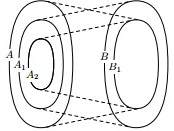
\includegraphics[height=5cm, width=\linewidth]{images/kantorbern1.jpg}
 \caption{Взаимные соответсвия между множествами}
 \end{minipage}
 \end{center}
 \end{figure}
 
 Теперь мы можем забыть про множество $B$ и его подмножества и доказывать такой факт:
 
 \textit{Если $A_2 \subset A_1 \subset A_0$ и $A_2 \sim A_0$, то все три множества
равномощны.}

 (Для единообразия мы пишем $A_0$ вместо $A$.)
 
 Пусть $f$ — функция, осуществляющая взаимно однозначное соответствие $A_0 \rightarrow A_2$ (элемент $x \in A_0$ соответствует элементу $f(x) \in A_2$). Когда $A_0$ переходит в $A_2$, меньшее множество $A_1$ переходит в какое-то множество $A_3 \subset A_2$ (см. рис. 2). Аналогичным образом само $A_2$ переходит в некоторое множество $A_4 \subset A_2$. При этом $A_4 \subset A3$, так как $A_1 \subset A_2$.

 \begin{figure}[h]
\begin{center}
\begin{minipage}[h]{0.4\linewidth}
 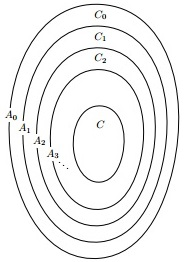
\includegraphics[height=5.3cm, width=\linewidth]{images/kantorbern2.jpg}
 \caption{Последовательные вхождения множеств}
 \end{minipage}
 \end{center}
 \end{figure}
 
 Продолжая эту конструкцию, мы получаем убывающую последовательность множеств
 
 \[A_0 \supset A_1 \supset A_2 \supset A_3 \supset A_4 \supset \ldots\]

 и взаимно однозначное соответствие $f : A_0 \rightarrow A_2$, при котором $A_i$ соответствует $A_{i + 2}$ (иногда это записывают так: $f(A_i) = A_{i+2}$). Формально можно описать $A_{2n}$ как множество тех элементов, которые получаются из какого-то элемента множества $A_0$ после $n$-кратного применения функции $f$. Аналогичным образом $A_{2n + 1}$ состоит из тех и только тех элементов, которые получаются из какого-то элемента множества $A_1$ после $n$-кратного применения функции $f$.
 
 Заметим, что пересечение всех множеств $A_i$ вполне может быть непусто: оно состоит из тех элементов, у которых можно сколько угодно раз брать $f$-прообраз. Теперь можно сказать так: множество $A_0$ мы разбили на непересекающиеся слои $C_i = A_i / A_{i+1}$ и на
сердцевину $C =\cap_i A_i$.

 Слои $C_0, C_2, C_4, \ldots$ равномощны (функция $f$ осуществляет взаимно однозначное соответствие между $C_0$ и $C_2$, между $C_2$ и $C_4$ и т.д.):

\[C_0 \xrightarrow{f} C_2 \xrightarrow{f} C_4 \xrightarrow{f} \ldots\]

То же самое можно сказать про слои с нечётными номерами:

\[C_1 \xrightarrow{f} C_3 \xrightarrow{f} C_5 \xrightarrow{f} \ldots\]

Можно ещё отметить (что, впрочем, не понадобится), что функция $f$ на множестве $C$ осуществляет его перестановку.

Теперь легко понять, как построить взаимно однозначное соответствие $g$ между $A_0$ и $A_1$. Пусть $x \in A_0$. Тогда соответствующий ему элемент $g(x)$ строится так: $g(x) = f(x)$ при $x \in C_{2k}$ и $g(x) = x$ при $x \in C_{2k + 1}$ или $x \in C$ (см. рис. 3)

\begin{figure}[h]
\begin{center}
\begin{minipage}[h]{0.4\linewidth}
 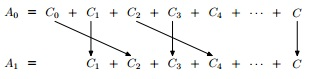
\includegraphics[height=2cm, width=\linewidth]{images/kantorbern3.jpg}
 \caption{Построение взаимно-однозначного соответствия}
 \end{minipage}
 \end{center}
 \end{figure}

\end{proof}

\section*{25. Теорема Поста: формулировка и доказательство.}

\begin{poste}

Если множества $A$ и $\overline{A}$ перечислимы, то множество A разрешимо.

\end{poste}

\begin{proof}

Алгоритм разрешения множества $A$ устроен так. Он исполняет
модифицированные алгоритмы перечисления множеств $A$ и $\overline{A}$ параллельно: один шаг работы алгоритма перечисления множества A, затем один шаг работы алгоритма перечисления $\overline{A}$ и так далее.

Вместо того, чтобы печатать очередной элемент, модифицированный алгоритм
перечисления запоминает его в списке элементов множества. (В любой момент исполнения алгоритма такой список конечен.)

Когда один из списков увеличивается, добавленный элемент сравнивается со входом $x$. Если обнаружено вхождение $x$ в список элементов множества $A$, то алгоритм разрешения останавливается и выдаёт результат $1$. Если обнаружено вхождение $x$ в список элементов множества $\overline{A}$, то алгоритм разрешения останавливается и выдаёт результат 0. В остальных случаях продолжается работа алгоритмов перечисления.

Докажем корректность алгоритма. Пусть $x \in A$. Тогда $x$ заведомо не входит в список элементов $\overline{A}$ и результат $0$ невозможен. С другой стороны, рано или поздно $x$ появится в списке элементов $A$, поэтому алгоритм выдаст результат $1$.

Аналогично рассуждаем в случае $x \notin A$.

\end{proof}

\section*{26. Разрешимые множества перечислимы.}

\statement{Если множество $S$ разрешимо, то оно перечислимо.}

\begin{proof}
Алгоритм перечисления множества $S$ использует алгоритм раз-
решения множества $S$. Он перебирает все числа, начиная с 0; для каждого числа
$n$ вычисляет индикаторную функцию $\chi S(n)$ и печатает число n, если полученное
значение равно 1.

            \begin{algorithm}
            \caption{Алгоритм перечисления множества S}
            \begin{algorithmic}[1]
            \Function{Print}{S(n)}
                \For{$n := 0 \ldots \infty$}
                    \If{$\chi_{S}(n) = 1$}
                        \State \textbf{print} n
                    \EndIf
                \EndFor
            \EndFunction
            \end{algorithmic}
            \end{algorithm}
            
Корректность такого алгоритма ясна из определений.
\end{proof}

\section*{27. Перечислимые множества являются множествами значений вычислимых функций.}

\sign{
    \
    
    $Comp$ -- клас вычислимых функций.
    
    $Dom\ Comp$ -- класс областей определения вычислимых функций.
    
    $Range\ Comp$ -- класс областей значения вычислимых функций.
    
    $Range^t\ Comp$ -- класс областей значения всюду определённых вычислимых функций.
    
    $\Sigma_1$ -- класс перечисоимых множеств.
}

\statement{$\Sigma_1 \subseteq Range\ Comp$}
        
        \begin{proof}
            По определению перечислимого множества, множество $S$ -- перечислимо, если существует такая вычислимая функция:
            
            \[
                f: \N \to \N\ 
                \begin{cases}
                    f(\N) = S \\
                    \text{Область определения} \ f \ \text{равна либо} \ \N, \text{либо} \ [n].
                \end{cases}
            \]
            
            Тогда очевидно, что перечислимые множества есть множества значений вычислимых функций.
        \end{proof}

\section*{28. Перечислимые множества являются множествами значений всюду определенных вычислимых функций.}

Cледствие Доказательств $27$, $29$ и $32$: $Range^t\ Comp \subseteq \Sigma_1 \subseteq Range\ Comp \subseteq Range^t\ Comp$. $29$ и $32$ приведены ниже.


\section*{29. Множества значений всюду определенных функций перечислимы.}


\statement{$Range^t\ Comp \subseteq \Sigma_1$}
        
        \begin{proof}
            Пусть $f(n)$ -- всюду определённая вычислимая функция. Построим алгоритм, перечисляющий множество её значений:
            
            \begin{algorithm}
            \caption{Алгоритм перечисления множества значений вычислимой функции}
            \begin{algorithmic}[1]
            \Function{PrintSet}{f(n)}
                \For{$n := 0 \ldots \infty$}
                    \State \textbf{print} f(n)
                \EndFor
            \EndFunction
            \end{algorithmic}
            \end{algorithm}
            
            Поскольку у множества значений вычислимой функции существует алгритм, его перечисляющий, то это множество перечилимо.
            
        \end{proof}

\section*{30. Множество значений всюду определенной вычислимой функции является областью определения вычислимой функции.}

\statement{$Range^t\ Comp \subseteq Dom\ Comp$}
        
        \begin{proof}
            Пусть $S = f(n)$ для некоторой всюду определённой функции $f$. Опишем алгоритм вычисления функции $g$, который получает на вход $x$: перебираем все числа, начиная с 0; для каждого числа $n$ вычисляем $f(n)$ и сравниваем с $x$; в случае равенства выдаём результат 1.
            
             \[
                g(x) =
                \begin{cases}
                    1, \text{если $x \in Rangef$} \\
                    \text{иначе не определена, так как для любого n выполняется $x \neq f(n)$}.
                \end{cases}
            \]
            
        Заметим, что мы доказали, что $g$ --- константна.
        \end{proof}

\section*{31. Область определения вычислимой функции является множеством значений вычислимой функции.}

\statement{$Dom\ Comp \subseteq Range\ Comp$}
        
        \begin{proof}
             Пусть $S$ — область определения некоторой вычислимой функции $f$, а $p$ --- номер программы, вычисляющей f. 
             
            Опишем алгоритм вычисления функции $g$ из $\mathbb N \times \mathbb N$ в $\mathbb N$ на входе $(x, t)$: вычисляем $F(p, x, t)$ и сравниваем с $1$; если $F(p, x, t) = 1$, то выдаём результат $x$, иначе не выдаём никакого результата.

            Если $x \in S$, то $x = g(x, t)$ для некоторого $t$. И обратно, если $x = g(x, t)$ для некоторого $t$, то $U(p, x)$ определена, а значит, определена и $f(x)$.

            Мы представили $S$ как множество значений функции от двух натуральных аргументов. Чтобы перейти к функциям одного аргумента, используем вычислимую биекцию $c : \mathbb N \times \mathbb N \to \mathbb N$ и выразим $S$ как $S = g \circ c^{-1}(N)$.
        \end{proof}

\section*{32. Непустое множество значений вычислимой функции является множеством значений всюду определенной вычислимой функции.}

\statement{$Range\ Comp \subseteq Range^t\ Comp$}
        
        \begin{proof}
            Пусть $S = f(n)$ для некоторой вычислимой функции $f$. Зафиксируем некоторое $a \in S$ (мы предполагаем, что множество $S$ непусто). 
            
            Функция $f$ не всюду определена и может не иметь вычислимого всюду определённого продолжения. Поэтому используем отладочную функцию. 
            
            Пусть $f(x) = U(p, x)$, где $U$ — некоторая универсальная вычислимая функция, для которой существует отладочная функция. Опишем алгоритм вычисления всюду определённой функции $g : \mathbb N \times \mathbb N \to \mathbb N$. На входе $(x, t)$ алгоритм вычисляет $F(p, x, t)$ и сравнивает результат с $1$. Если $F(p, x, t) = 1$, то алгоритм выдаёт $U(p, x)$. В противном случае результат равен $a$. 
            
            По определению отладочной функции из $F(p, x, t) = 1$ следует, что $U(p, x)$ определена. Поэтому функция g всюду определена. Её множество значений совпадает с $S$. В одну сторону: если $y = g(x, t)$, то $y = a \in S$ или $y = U(p, x) = f(x) \in S$. В другую: пусть $y = f(x) = U(p, x)$. На паре $(p, x)$ функция $U$ определена, поэтому для некоторого $t$ значение отладочной функции $F(p, x, t) = 1$. Но тогда $y = g(x, t)$. Мы представили S как множество значений всюду определённой функции от двух натуральных аргументов. Чтобы перейти к функциям одного аргумента, используем вычислимую биекцию $c : \mathbb N \times \mathbb N \to \mathbb N$ и выразим $S$ как $S = g \circ c^{-1}(\mathbb N)$.
        
        \end{proof}

\section*{33. Пример перечислимого неразрешимого множества}

\begin{theorem}
    Существует перечислимое неразрешимое множество.
\end{theorem}

\begin{proof}
    Рассмотрим вычислимую функцию $f(x)$, не имеющую всюду определённого вычислимого продолжения. Её область определения $F$ будет искомым множеством. В самом деле, $F$ перечислимо (по одному из определений перечислимости). Если бы $F$ было разрешимо, то функция
    
    \[
        g(x) =
        \begin{cases}
            f(x), \text{если $x \in F$} \\
            0, \text{если  $x \notin F$}.
        \end{cases}
    \]
    
    была бы вычислимым всюду определённым продолжением функции $f$ (при вычислении $g(x)$ мы сначала проверяем, лежит ли $x$ в $F$, если лежит, то вычисляем $f(x)$).
\end{proof}

Пусть $U$ — некоторая универсальная функция. Обозначим через $H$ множество

\[
    \{x : U(x,\ x)\ \text{определена}\}.
\]

\statement{$H$ перечислимо, но неразрешимо}

\begin{proof}
Множество $H$ является областью определения вычислимой функции $x \to U(x,\ x)$. Поэтому оно перечислимо.
    
Неразрешимость доказывается диагональным методом. Предположим, что
$H$ разрешимо. Рассмотрим такой алгоритм вычисления функции $f$: на входе $x$ он
вызывает алгоритм разрешения множества $H$ для $x$. Если $x \in H$, то алгоритм не даёт никакого результата, а если $x \notin H$, то выдаёт результат $1$.

Пусть $p$ — номер функции $f$ в универсальной нумерации, то есть $f(x) = U(p,\ x)$.

Предположим, что $p \in H$. Тогда алгоритм вычисления $f$, описанный выше, не
выдаёт никакого результата, то есть $f(p) = U(p,\ p)$ не определено. По определению множества $H$ это означает, что $p \notin H$.

Если $p \notin H$, то алгоритм вычисления $f$ даёт результат $1$, то есть $1 = f(p) = U(p,\ p)$. Следовательно, $p \in H$.

Пришли к противоречию. Значит, множество $H$ неразрешимо.

\end{proof}

\section*{34. Невозможность универсальной нумерации всюду определенных вычислимых функций: формулировка и доказательство.}

    Были введены универсальные нумерации вычислимых
    функций. А может быть можно ввести аналогичную
    нумерацию для всюдуопределённых функций?
    
    Вопрос: существует ли такая всюдуопределённая
    функция $V(p, x)$, что для любой всюдуопределённой
    функции $f(x)$ существует номер $p$ такой, что
    $\forall x \in N f(x) = V(p, x)$?

\begin{theorem}
    Не существует универсальной нумерации всюду определённых вычислимых функций.
\end{theorem}

\begin{proof}
    Расмотрим функции вида $V(p,x)$, всюду определённые
    (как раз наша потенциальная нумерация).
    
    Воспользуемся диагональным методом, построив (мысленно) таблицу таких функций.
    
    Возьмём $f(x) = V(x,x) + 1$. $f(x)$ вычислима? Да.
    Так как $V(x, x)$ всюдуопределена, то $f(x)$ тоже
    всюдуопределена.
    
    Однако (как ни странно!) такой функции в нумерации гарантированно нет. Почему? Пусть $f(x)$ имеет
    в такой нумерации номер $p$. Тогда посмотрим,
    чему равно $f(p)$:
    \[
    f(p) = V(p, p)
    \]
    и с другой стороны:
    \[
    f(p) = V(p, p) + 1
    \]
    
    $V(p, p) = V(p, p) + 1$. Противоречие!
\end{proof}

\section*{35. Функция вычислима тогда и только тогда, когда ее график перечислим.}

\begin{theorem}
    Функция вычислима тогда и только тогда, когда её график перечислим.
\end{theorem}

\begin{proof}
Пусть $f(x)$ вычислима. Перечислим его график алгоритмом:
\begin{algorithm}
        \caption{Алгоритм перечисления графика функции}
        \label{algo:35_task_proof}
        \begin{algorithmic}
            \Function{count\_graph}{x}
                \For{$i := 0..\infty$}
                \State $(x, t) = \pi(i)$
                \State \# запустить $f(x)$ на $t$ тактов
                \If{$f(x)$ остановилась}
                    \State print $(x, f(x))$
                \EndIf
                \EndFor
            \EndFunction
        \end{algorithmic}
\end{algorithm}

Пусть теперь $x \in Dom(f)$ тогда $f(x)$ останавливается
на каком-то $t$, а значит точка $(x, f(x))$ будет перечислена. Если $x \notin Dom(f)$ тогда $f(x)$ не
останавливается при любом $t$, а значит эта точка
перечислена не будет. 

$\pi: \N \to \N \times \N$ -- вычислимая биекция (сущетвование доказывалось ранее).

Пусть график $G = \{(x,\ y) :\ y = f(x)\}$ перечислим. Тогда следующий алгоритм
вычисляет $f$: на входе $x$ запускаем перечисление элементов графика, когда найден очередной элемент $(y,\ z)$, проверяем $x = y$, в случае равенства выдаём результат $z$.

Из определения графика ясно, что на входе $x$ такой алгоритм может выдать
лишь результат $f(x)$. С другой стороны, если $x$ принадлежит области определения $f$, то пара $(x,\ f(x))$ рано или поздно будет перечислена. В этот момент алгоритм и выдаст результат $f(x)$.

\end{proof}

\section*{36. Перечислимые множества — это в точности проекции разрешимых.}

\begin{theorem}
    Перечислимые множества — это в точности проекции разрешимых.
\end{theorem}

\begin{proof}
Проекция пустого множества пуста. Дальше рассматриваем только непустые множества.
    
Пусть $D \subseteq \N \times \N$ разрешимо, $(a,\ b) \in D$. По определению, индикаторная функция $\chi_D$ вычислима. Но тогда вычислима и функция

\[
    f: (x,\ y) =\  
    \begin{cases}
        x,\ \text{если} \chi_D(x,\ y) = 1 \\
        a,\ \text{в противном случае}
    \end{cases}
\]

для которой $f(\N \times \N) = Pr\ D$. Поэтому $Pr\ D$ перечислимо.

Пусть $S$ — перечислимо. Тогда $S$ — область определения некоторой вычислимой
функции $f$, которая имеет номер $p$ в универсальной нумерации. Построим такое
множество:

\[
    D = \{(x,\ t) :\  F(p,\ x,\ t) = 1\}.
\]

Докажем, что $Pr\ D = S$. Пусть $x \in S$. Это значит, что на $x$ функция $f$ определена, тем самым определена и функция $U(p,\ x)$. Но тогда по определению отладочной функции $F(p,\ x,\ t) = 1$ для некоторого $t$, то есть $x \in Pr\ D$.

В обратную сторону аналогично: если $x \in Pr\ D$, то для некоторого $t$ выполняется $F(p,\ x,\ t) = 1$, то есть $U(p,\ x) = f(x)$ определена. Таким образом, $x \in S$.

\end{proof}

\section*{37. Пример вычислимой функции без всюду определенного вычислимого продолжения.}

Определим $\overline{h_U}$ как

    \[
        \overline{h_{U}}(x) =
        \begin{cases}
            1, \text{если $U(x, x) = 0$} \\
            0, \text{если $U(x, x)$ определена и $U(x, x) \neq 0$ }.
        \end{cases}
    \]

Эта функция вычислима: подадим на вход алгоритма, вычисляющего $U$, пару аргументов $(x, x)$; после остановки этого алгоритма выдадим 1, если результат вычисления $U$ равен $0$, и $0$ в противном случае. Если $U(x, x)$ не определена, то данный алгоритм также не выдаёт никакого результата.

\begin{theorem}
    У $\overline{h_U}$ нет всюду определённого вычислимого продолжения (нет функции, доопределяющей $\overline{h_U}$ на всей области определения).
\end{theorem}

\begin{proof}
    
    Доказываем от противного. Пусть $g(x)$ --- всюду определённое вычислимое продолжение функции $\overline{h_U}$. Выберем такое $p$, что $g(x) = U(p, x)$ и придём к противоречию аналогично доказательству теоремы о невычислимости $H$. Так как $g(x)$
    всюдуопределённая, то и в точке $p$ она определена. А значит $U(p, p)$ определена, при этом $g(p) = \overline{h_U}(p)$ (так как $g$ -- продолжение $\overline{h_U}$). 
    Возможны два случая:
    \begin{enumerate}
        \item $U(p, p) = 0 \implies g(p) = 0, g(p) = 
        \overline{h_U}(p) \implies 
        \overline{h_U}(p) = 0 \implies
        U(p, p) \neq 0$. Противоречие
        \item $U(p, p) \neq 0 \implies g(p) \neq 0,
        g(p) = \overline{h_U}(p) \implies
        \overline{h_U}(p) \neq 0 \implies
        \overline{h_U}(p) = 1$ (так как никаких других
        значений $\overline{h_U}$, кроме $0$ и $1$ не принимает). А это значит, что $U(p,p) = 0$. 
        Противоречие.
    \end{enumerate}
    
    В обоих случаях получили противоречие, а значит
    и такого дополнения нет.

\end{proof}

\section*{38. Доказательство теоремы Успенского–Райса.}

Cледствие из теоремы о неподвижной точке:

\begin{rec}
    Для любой вычислимой функции $V(n,\ x)$ и главной универсальной
    функции $U(n, x)$ существует $q$ такое, что:

    \[
        V(q,\ x) = U(q,\ x).
    \]

\end{rec}

\begin{proof}
    Найдем $s(n): V(n, x) = U(s(n), x)$. $s(n)$ -- всюдуопределённая.
    Тогда (по теореме о неподвижной точке)
    $\exists q : V(q, x) = U(s(q), x) = U(q, x)$.
\end{proof}

Пусть есть некоторое свойство, которое мы хотим проверить
для некоторой функции. 

Формально:
Пусть $\{f:\N\to\N\}$ -- множество вычислимых функций. 
Разделим его на два непересеающихся подмножества $A$ и $\overline{A}$.
\[
\{f\ |\ f:\N\to\N\} = A \cup \overline{A}
\]
$A$ -- множество тех функций, для которых выполняется некое свойство,
$\overline{A}$ -- множество тех функций, для которых это свойство не выполняется.

Возьмём некоторую универсальню функцию $U(p,\ x)$.

Обозначим за $P_A$ множество всех $p$ таких, что $U(p,\ x) \in A$.
\[
P_A = \{p\ |\ U(p, x) \in A\}
\]

Тогда вопрос можно поставить так: разрешимо ли множество
программ, удовлетворяющих нашему свойству? На этот вопрос и отвечает теорема
Успенского-Райса:
\begin{usp-rais}
   Если $A$ -- нетривиально ($A \neq \oslash,\ \overline{A} \neq \oslash$), а $U(q,\ x)$ -- главная универсальная функция, то множество $P_A$ неразрешимо.
\end{usp-rais}
Введём для удобства ещё функции $\varepsilon \in \overline{A}$ (нигде не 
определённая) и $\xi \in A$ (какая-то функция, удовлетворяющая условию).
Сделать это можно по аксиоме выбора.

Если $A$ -- это множество нигде не определённых функций, то поменяем их
местами так как $P_A$ разрешимо тогда и только тогда, когда его
дополнение разрешимо.

\begin{proof}[Доказательство 1]
    Пусть $P_A$ разрешимо. Тогда существует всюдуопределённая
    характеристическая функция $\chi_{P_A}$. 
    Построим алгоритм на странице \pageref{algo:usp-rais-proof1} 
    (алгоритм \ref{algo:usp-rais-proof1}).
    \begin{algorithm}
        \caption{Алгоритм, создающий противоречие для разрешимости $P_A$ в док-ве 1}
        \label{algo:usp-rais-proof1}
        \begin{algorithmic}
            \Function{problem}{x}
                \If{$\chi_{P_A} = 0$}
                    \State \Return $\xi(x)$
                \Else 
                    \State \Return $\varepsilon(x)$.
                \EndIf
            \EndFunction
        \end{algorithmic}
    \end{algorithm}
    
    Он имеет некоторый номер $p$ (который использован в программе) в $U$.
    \begin{itemize}
            \item $p \in P_A$. Тогда $U_p(x) = \varepsilon(x)$,
                но $\varepsilon(x) \in \overline{A} \implies
                p \notin P_A$. Противоречие.

            \item $p \notin P_A$. Тогда $U_p(x) = \xi(x)$, но
                $\xi(x) \in A \implies p \in P_A$. Противоречие.
    \end{itemize}
    Значит алгоритма разрешения не существует.

    Может показаться, что использование номера программы в ней самой недопустимо,
    однако по свойству рекурсии это делать абсолютно законно.
\end{proof}

\begin{proof}[Доказательство 2]
    Пусть есть алгоритм, который строит алгоритм по номеру из шаблона
    (функция $\varphi : n \mapsto p_n$). Алгоритм выглядит так, как показано
    на странице \pageref{algo:usp-rais-proof2} (алгоритм \ref{algo:usp-rais-proof2}).

    \begin{algorithm}
        \caption{Шаблон алгоритма $p_n$ для функции $\varphi$ в док-ве 2}
        \label{algo:usp-rais-proof2}
        \begin{algorithmic}
            \Function{problem}{x}
                \State $U(n, n)$
                \State \Return $\xi(x)$
            \EndFunction
        \end{algorithmic}
    \end{algorithm}

    Пусть $H = \{ n\ |\ U(n, n) \text{ останавливается} \}$.
    Рассмотрим два случая:
    \begin{enumerate}
        \item $n \in H \implies U(p_n, x) = \xi(x)$.
        \item $n \notin H \implies U(p_n, x) = \varepsilon(x)$.
    \end{enumerate}
    Что это значит? Это значит, что мы выразили (по факту)
    одну характеристическую функцию через другую:
    \[ \chi_H(n) = (\chi_{P_A} \circ \varphi)(n) \]
    \[ n \in H \iff p_n \in P_A \]

    Если $\chi_{P_A}$ вычислима, то вычислима и $\chi_H$, однако это не так.

    Так как функция $U$ -- главная, то $\varphi$ представима в виде функции
    от двух аргументов $V(n, x)$ (номера шаблона и аргумента).
    \[ U(p_n, x) = V(n, x) = U(s(n), x) \]

    Значит $\chi_{P_A}$ не является вычислимой.

\end{proof}

\section*{39. Доказательство теоремы о неподвижной точке.}

\begin{point}
    Пусть $U$ -- главная универсальная функция, $h(n)$ -- любая всюду определённая вычислимая функция. Тогда:
    
    \[
        \exists\ q \ : \ U(q,\ x) = U(h(q),\ x).
    \]
\end{point}

Честно сказать, не все учёные понимают эту теорему, однако её можно объяснить неформально
так: для любой программы на любом универсальном языке существует ещё одна программа,
которая делает то же самое (то есть программы совпадают).

\begin{proof}
    Для начала найдем такую функцию $f(p): \forall g(p) - \text{вычислимой } 
    \exists p: f(p) = g(p)$. В действительности, она существует, вот например:
    $f(p) = U(p, p)$. Тогда $g(p)$ тоже имеет какой-то номер $q$ и тогда
    $g(q) = U(q, q) = f(q)$.

    Рассмотрим функцию $V(p, x) = U(f(p), x)$. Тогда $V(p, x)$ -- универсальная,
    ведь если была функция $\varphi$ с номером $k$, тогда в некоторой точке $f(p)$
    принимает значение $k$ и $\varphi(x) = U(f(p), x) = V(p, x)$. 
    
    По определению главной универсальной функции $V(p, x) = U(s(p), x)$.

    Соберём все вместе и получим: $U(f(p), x) = V(p, x) = U(s(p), x)$. Заметим,
    что $f(p)$ не обязана быть всюдуопределённой, а $s(p)$ уже всюдуопределена.

    Тогда вспомним про нашу функцию $h(n)$ из условия и введём функцию $g(p) = h(s(p))$.
    Тогда (по построению функции $f$): $\exists p : g(p) = f(p)$.

    Опять же, собираем всё вместе:
    \[
    \exists p : U(s(p), x) = V(p, x) = U(f(p), x) = U(g(p), x) = U(h(s(p)), x)
    \]
    Пусть $q = s(p)$. Тогда:
    \[
    \exists q : U(q, x) = U(h(q), x)
    \]
\end{proof}

\section*{40. Композиция функций, вычислимых на машине Тьюринга, вычислима на машине Тьюринга.}

\begin{theorem}
    Пусть $f : B^{*} \to B^{*},\ g : B^{*} \to B^{*}$ вычислимы МТ. Тогда $f \circ g$ также вычислима МТ.
\end{theorem}

\begin{proof}
    
    Результат работы одного алгоритма можно подать на вход другого алгоритма.

    Пусть $M_1$ вычисляет $g$, а $M_2$ вычисляет $f$. Тогда МТ, которая состоит из последовательного соединения блоков $M_1$ и $M_2$ вычисляет $f \circ g$.
    
    Если первая машина $M_1$ заканчивает работу, оставляя на ленте
    только полезный результат и ничего больше, то тогда определён результат вычисления МТ, так как на ленте не останется \textit{мусора}, изменяющего работу машины.
    
    Докажем тогда лемму \textit{об уборке мусора}
    \ 
    
    \begin{fulllemma}Пусть машина $M$ вычисляет функцию $f$. Тогда существует такая машина $M'$, которая вычисляет ту же функцию, но финальная конфигурация которой на любом входе $w$ из области определения $f$ имеет вид $q_f f(w)$.
    \end{fulllemma}
    
    \begin{proof}
        Машина $M'$ будет последовательным соединением четырёх машин.
        
        \begin{enumerate}
            \item Первая машина $M_1$ преобразует начальную конфигурацию $q'_0w$ в конфигурацию $\triangleleft q_0w \triangleright$, где $q_0$ — начальное состояние машины $M$.
            \item Вторая машина $M_2$ работает так же, как исходная машина $M$, но сохраняет окаймление конфигурации символами $\triangleleft,\ \triangleright$.
            \item Третья машина $M_3$ стирает символы слева от положения головки в финальной конфигурации машины $M_2$.
            \item Четвёртая машина $M_4$ стирает символы справа от последнего символа результата работы $M_2$ и возвращает головку в ту ячейку, в которой она была при остановке машины $M_2$.
        \end{enumerate}

        Как ясно из этого описания, при корректной реализации каждой из этих четырёх машин их соединение $M'$ удовлетворяет искомому свойству.

        Опишем реализации этих четырёх машин.
        
        Машина $M_1$ последовательно выполняет следующие шаги:
        
        \begin{enumerate}
            \item сдвинуться на одну ячейку влево, записать в неё символ $\triangleleft$
            \item сдвинуться до первого пустого символа справа
            \item записать символ $\triangleright$
            \item сдвинуться до символа $\triangleleft$ слева
        \end{enumerate}
        
        Таблица переходов машины $M_2$ совпадает с таблицей переходов исходной машины $M$ за исключением работы на добавленных символах $\triangleleft,\ \triangleright$. На символе $\triangleleft$ машина выполняет следующие такты работы:
        
        \begin{enumerate}
            \item записать пустой символ, сдвинуться влево и перейти в состояние $\overline{q}$ 
            \item  записать символ $\triangleleft$, сдвинуться вправо перейти в состояние $q$
        \end{enumerate}
        
         Работа $M_2$ на символе $\triangleright$ устроена аналогично (разумеется, символ переносится вправо).
        
        \begin{figure}[h]
            \begin{center}
            \begin{minipage}[h]{0.6\linewidth}
                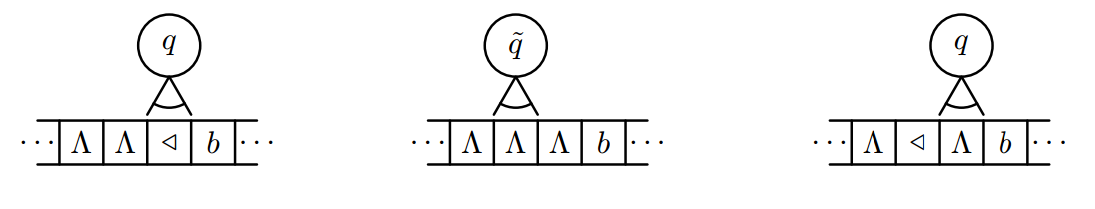
\includegraphics[height=2cm, width=\linewidth]{images/MTboarder.png}
                \caption{Сдвиг левого ограничителя рабочей зоны}
            \end{minipage}
            \end{center}
        \end{figure}
        
        Как видно из описания, количество состояний у машины $M_2$ в два раза больше, чем у исходной машины $M$, а работа при чтении добавленных символов окаймления устроена так, что машина переносит символ окаймления на одну ячейку вне рабочей зоны, возвращается назад и продолжает работу как исходная машина $M$. Поэтому машина $M_2$ закончит работу, имея слева и справа от рабочей зоны символы $\triangleleft,\ \triangleright$.
        
        Опишем теперь устройство машины $M_3$. Она начинает работу в одном из финальных состояний $q_f$ исходной машины $M$. Работа машины $M_3$ разбивается на следующие шаги:
        
        \begin{enumerate}
            \item пометить текущую ячейку, сдвинуться влево и перейти в состояние $q_l$
            \item идти влево до символа $\triangleleft$, заменяя символ в каждой ячейке на пустой символ
            \item на символе $\triangleleft$ записать пустой символ и перейти в финальное состояние $q_r$
        \end{enumerate}

        Второй шаг реализуется такой таблицей переходов:
        
        \[
           \delta(a,\ q_l) = (\Lambda,\ q_l, -1),\ a \neq \triangleleft
        \]
        
        Ясно, что в результате работы машины $M_3$ все символы слева от результата работы исходной машины $M$ будут заменены на пустые.
        
        Последняя машина $M_4$ должна убирать мусор справа от результата работы исходной машины. Она начинает работу в состоянии $q_r$ (финальном состоянии предыдущей машины) и исполняет следующие шаги:
        
        \begin{enumerate}
            \item сдвинуться вправо до помеченной ячейки
            \item сдвинуться вправо до пустого символа (быть может, помеченного)
            \item идти вправо до символа $\triangleright$, заменяя символ в каждой ячейке на пустой символ
            \item на символе $\triangleright$ записать пустой символ
            \item идти влево до помеченной ячейки
            \item убрать пометку и остановиться
        \end{enumerate}

        По завершении последовательной работы машин $\{M_1,\ M_2,\ M_3,\ M_4\} = M'$ финальная конфигурация на входе $w$ из области определения $f$ как раз будет иметь вид $q_f f(w)$.
        
    \end{proof}
    
    По лемме об уборке мусора каждая вычислимая на МТ функция вычислима машиной, которая в конце работы оставляет на ленте только результат работы.
    
    Машину $M_1$, вычисляющую $g$, заменяем на "усовершенствованную" машину $M_1'$, вычисляющую ту же функцию $g$, но при этом не оставляющую "мусора". Также заменим $M_2$ на аналогичную $M_2'$. Последовательно соединяем $M_1'$ и $M_2'$, вычисляющую $f$, и получаем композицию машин $M_2' \circ M_1'$, вычисляющую композицию функций $f \circ g$.
    
    Тогда ясно, что последовательное соединение любого количества таких "усовершенствованных" машин вычисляет композицию функций, вычислимых этими машинами.
    
\end{proof}

\end{document}